\documentclass[crop,class=article]{standalone}
%----------------------------Preamble-------------------------------%
\usepackage{tikz}                   % Drawing/graphing tools.
%--------------------------Main Document----------------------------%
\begin{document}
    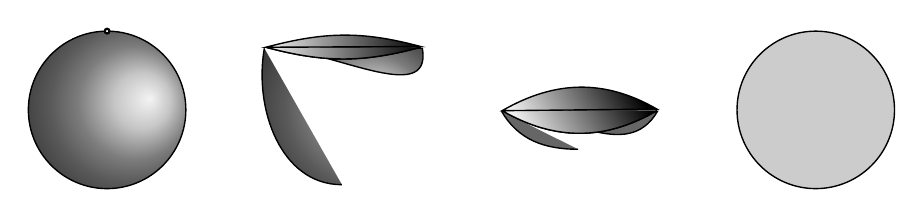
\begin{tikzpicture}[%
        scale=1,
        line width=0.5pt,
        sphereshade/.style={
            ball color=gray!60!white,
            draw=black,
            shading angle=240
        }
    ]
        \begin{scope}[%
            every node/.style={%
                inner sep=0pt,
                outer sep=0pt
            }
        ]
            % Points for the Second Blob.
            \node at (-1,-0.95) (a) {};
            \node at (-2,0.8) (b) {};
            \node at (0, 0.8) (c) {};

            % Points for the Third Blob.
            \node at (2,-0.5) (d) {};
            \node at (1,0) (e) {};
            \node at (3,0) (f) {};
        \end{scope}

        % First blob (Sphere).
        \filldraw[sphereshade] (-4,0) circle (1);

        % North pole of the sphere is missing.
        \filldraw[white, draw=black, thick]
            (-4,1) circle (0.3mm);

        % Draw the second blob
        \draw[sphereshade]
            (a) to [out=180,in=-100] (b) 
                to [out=-15,in=-165] (c)
                to [out=-80,in=0] cycle;
        \draw[left color=white!90!gray,right color=black]
            (b) to [out=-15,in=-165] (c)
                to [out=165,in=15] cycle;

        % Draw the third blob
        \draw[fill=black!20!gray]
            (d) to [out=180,in=-60] (e) 
                to [out=-30,in=-150] (f)
                to [out=-120,in=0] cycle;

        \draw[
            left color=black,
            right color=white!90!gray,
            shading angle=300
        ]
            (e) to [out=-30,in=-150] (f)
                to [out=150,in=30] cycle;

        % Draw the fourth blob (Circle)
        \filldraw[%
            draw=black,
             fill=white!60!gray
        ] (5,0) circle (1);
    \end{tikzpicture}
\end{document}